\documentclass{ximera}  


\title{The First Activity}  


\begin{document}  
\begin{abstract}  
This activity was created with Ximera.
\end{abstract}  
\maketitle  




    \begin{image}
      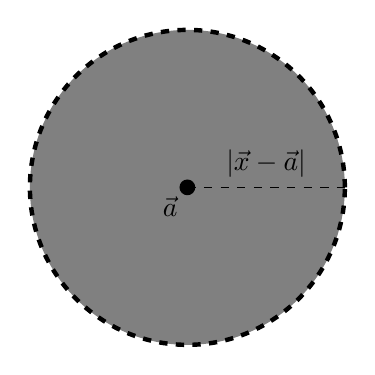
\begin{tikzpicture}
        \draw[ultra thick,dashed,fill=gray] (0,0) circle (2cm);
        \draw[draw=none,fill=black] (0,0) circle (.1cm);
        \draw[dashed] (0,0)--(2,0);
        \node[above] at (1,0) {$|\vec{x}-\vec{a}|$};
        \node[below left] at (0,0) {$\vec{a}$};
      \end{tikzpicture}
    \end{image}

\begin{onlineOnly}
  \[
  \graph{(sin(a t + d),sin(b t)}
  \]
\end{onlineOnly}


\begin{onlineOnly}
  \begin{center}
    \desmos{zwywds7med}{800}{600}
  \end{center}
\end{onlineOnly}

\begin{onlineOnly}
  \begin{center}
    \desmos{9gpht6dcqq}{800}{600}
  \end{center}
\end{onlineOnly}


\begin{onlineOnly}
  \begin{center}
    \geogebra{SqTP7Ubh}{800}{600}
  \end{center}
\end{onlineOnly}


\begin{onlineOnly}
  \begin{center}
    \geogebra{SRyzj9SD}{800}{600}
  \end{center}
\end{onlineOnly}

\begin{onlineOnly}
  \begin{center}
    \geogebra{QxdFYYMG}{800}{600}
  \end{center}
\end{onlineOnly}

\begin{onlineOnly}
  \begin{center}    
    \geogebra{h6qeZNva}{800}{600}
  \end{center}
\end{onlineOnly}


\begin{onlineOnly}
  \begin{center}    
    \geogebra{GyCgxY8c}{800}{600}
  \end{center}
\end{onlineOnly}


\begin{onlineOnly}
  \begin{center}    
    \geogebra{QZdktQMQ}{800}{600}
  \end{center}
\end{onlineOnly}








\[
\pm 6
\]

Here I have an array:
\[
\begin{array}{|c|c|}
  1 & 2 \\
  3 & 4
\end{array}
\]

here is a broken array

\[
\begin{array}{|c|c|}
  1 & 2 \\
  
  3 & 4
\end{array}
\]


This activity is about showing answer types.
\begin{problem}  
  Choose the best place to work on mathematics.  
  \begin{multipleChoice}  
    \choice{At the library}  
    \choice[correct]{At the cafe}  
    \choice{In your office}  
  \end{multipleChoice}
\end{problem}


\begin{problem}  
  Which of the following numbers are even?  
  \begin{selectAll}  
    \choice[correct]{$2$}  
    \choice{$1$}  
    \choice[correct]{$-4$}  
    \choice[correct]{$0$}  
  \end{selectAll}  
\end{problem}


\begin{problem}  
  $3\times 2 = \answer{6}$  
\end{problem} 

\begin{problem}  
  $\frac{\partial}{\partial x} x^2\sin(y) =  \answer{2x\sin(y)}$  
\end{problem} 

\begin{problem}
  Can you fill-in the blanks?
  \[
  2^{\answer{3}} = 8
  \]
  \begin{problem}
    \[
    \log_2(8) = \answer{3}
    \]
  \end{problem}
\end{problem}

\begin{problem}
  Can you fill-in the blanks?
  \[
  \int_{\answer{1}}^{\answer{3}}5 \, d x = 10
  \]
  \begin{hint}
    The lower bound of integration is $1$.
  \end{hint}
\end{problem}



\begin{problem}
  Tell us about yourself:
  \begin{freeResponse}
  \end{freeResponse}
\end{problem}


\end{document} 
